\section{Foundational Concepts}
\label{sec:concepts}

Our system, \texttt{T-REX} (or the Teleo-Reactive EXecutive) is an
adaptive, artificial intelligence based controller and provides
general framework for building reasoning systems for real-world
autonomous vehicles. At MBARI \texttt{T-REX} is used for AUV control;
another instantiation of the system is being used for control of a
terrestrial personal robot \cite{pr2, Meeussen:2010dn}. The development of
\texttt{T-REX} has been targeted at surveying a number of
oceanographic features which are dynamic and unpredictable
spatio-temporally. Typically this requires our AUVs to balance the
goals of coverage spatially while opportunistically following features
of scientific interest and to do so while being operationally aware of
its own limitations in terms of resources (typically the battery state
of charge) and overall proximity to other observational assets for
obtaining scientific ground-truth. We are therefore interested in
representational frameworks that allow robots to pursue long-term
objectives while choosing short-term gain and can gracefully deal with
exogenous or endogenous change.

To enable this responsiveness to external observations, the agent has
to be able to synthesize plans insitu and to re-plan. We use a
temporal constraint-based planner \eu with a demonstrated legacy of
having flown on NASA space missions \cite{jonsson00,bresina05,
  barreiro09}. Our autonomy architecture brings three key innovations
for AUV adaptation: the use of flexible plan representations,
compositional control with the use of partitioned networks and
off-line learning to inform insitu environmental state estimation. In
this section we detail some of the key concepts relevant to flexible
plan representation. Section \ref{sec:arch} has details the
\texttt{T-REX} partitioned architecture and estimation driven vehicle
adaptation.

\eu uses a domain model written in a declarative language (NDDL: New
Domain Description Language), together with initial conditions and
goals also specified in NDDL, to construct a set of temporal relations
that must be true at the start time. These models include assertions
about the physics of the vehicle, i.e how it responds to external
stimulus and internally driven goals. By propagating these relations
forward using Simple Temporal Networks \cite{dechter91} and applying
goal constraints, \eu can select a set of conditions that should be
true in the future, where some of these conditions will correspond to
actions the agent must take. The planner can backtrack and try another
path during search if a goal cannot be reached while being capable of
discarding unachievable goals.

Traditionally robot execution has relied on dispatching commands at
precise times. Such linear sequences of precisely timed commands give
no ability to adjust execution on the basis of sensory
information. Although some commands can issue tests on sensor
readings, these tests have the objective of verifying whether expected
execution conditions are occuring. If not, the state of the system is
declared off-nominal and execution of the sequence of commands is
interrupted. More recently, executives have been proposed and
implemented that significantly broaden the way robots can be commanded
\cite{mus98,alami:1998p820}. For example, the Remote Agent executive
interpreted a \textit{temporally flexible plan} which represents each
start time as a variable and contains an explicit network of bounded
delay constraints between such variables.

\begin{figure}[!t]
\centering
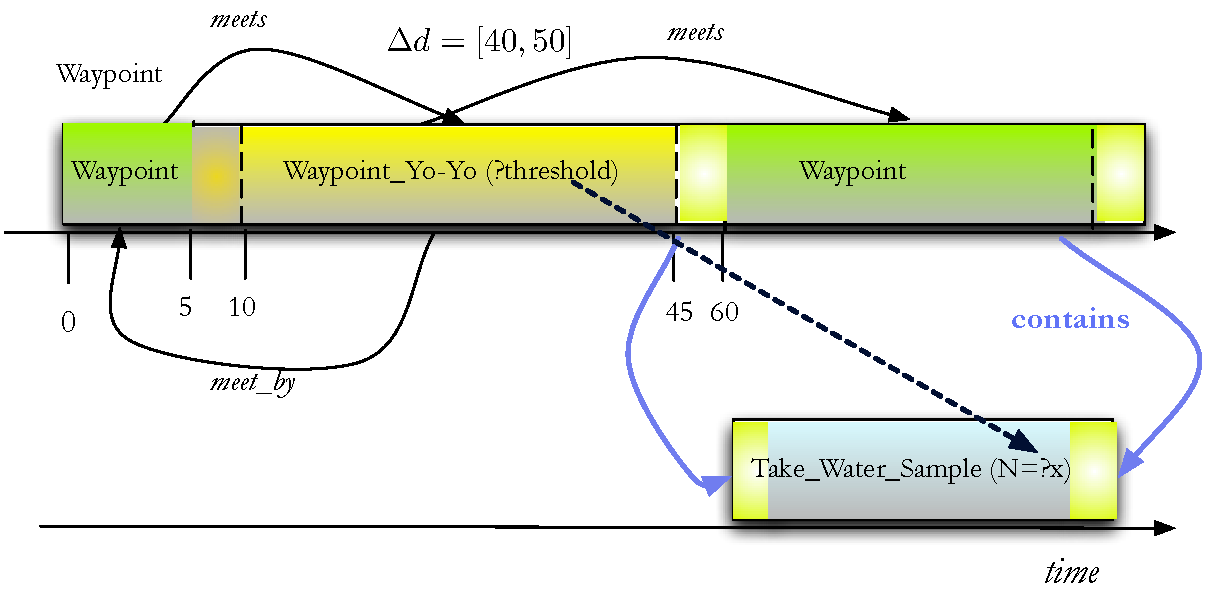
\includegraphics[scale=0.35]{figs/flexible-timelines.pdf}
\caption{\small Tokens with flexible temporal intervals and parametric
  constraints between tokens. This example shows the triggering of a
  water sampler based on a feature threshold while the vehicle
  Yo-Yo's. The \texttt{Waypoint\_Yo-Yo} token has a flexible duration,
  start \& end times.}
\label{fig:flex-timelines}
\vskip+0.1cm
\end{figure}

\eu uses a \emph{state variable} representation to describe the
evolution of state over time. The instantiated history of such state
variable evolution over a temporal horizon we call \emph{timelines}
and which represent a single thread in the execution of a concurrent
system. At any given time each thread can execute a single procedure.
Thus each timeline consists of a sequence of procedures which
encapsulate and describe state evolution; we call these instantiated
atomic entities \emph{tokens}.  A token therefore describes a
procedure invocation, the state variables on which it can occur, the
parameter values of the procedure, and the time values defining the
interval. We allow encapsulation of uncertainty within these tokens
with a range of start and end times and parameters, all of which are
encoded as variables. A constraint solver in turn manipulates these
variables defined in a \eu domain model. For example, consider
a scientific need to take a water samples 100 meters from a hotspot
while an AUV is performing a Yo-Yo in the water-column. Two samples
are needed if the feature's signal is above a threshold; one
otherwise. The token that is capturing the sensory threshold has a
parametric constraints to the token which fires the requisite water
sampler. In addition, the start time of the water sampling procedure
is highly dependant on the variability of sub-sea currents and actual
speed of the vehicle. Therefore a number of values are possible for
the start times and duration of the sampling all of which are valid
combinations for desired outcomes.

Unlike a traditional fixed time-tagged command sequences, such
flexible plans leave room for adaptation at execution time. When the
executive considers when to start a task, it propagates information
through the constraint network, computes a time bound for the
variable, selects an actual execution time within the bound, and
starts the task at that time. Temporally flexible plans therefore,
express a \textit{range of possible outcomes} of the robots
interaction with the environment within which the executive can elect
at run time the most appropriate one for the actual execution
conditions. The fact that constraints are explicitly represented
ensures that through constraint propagation the executive will respect
global limits expressed in the plan (e.g., don't start a task until a
certain condition has been satisfied but still satisfying some global
deadline). Such flexibility is critical when dealing with dynamic
ocean conditions where precise timing of a robotic action might be
indeterminate. Further, the advantage of flexibility can be contrasted
with the consequences of the intrinsic inflexibiliy of traditional
command sequences. Because they are inflexible, sequences must
necessarily be designed considering worst case scenarios.


\begin{figure}
\centering
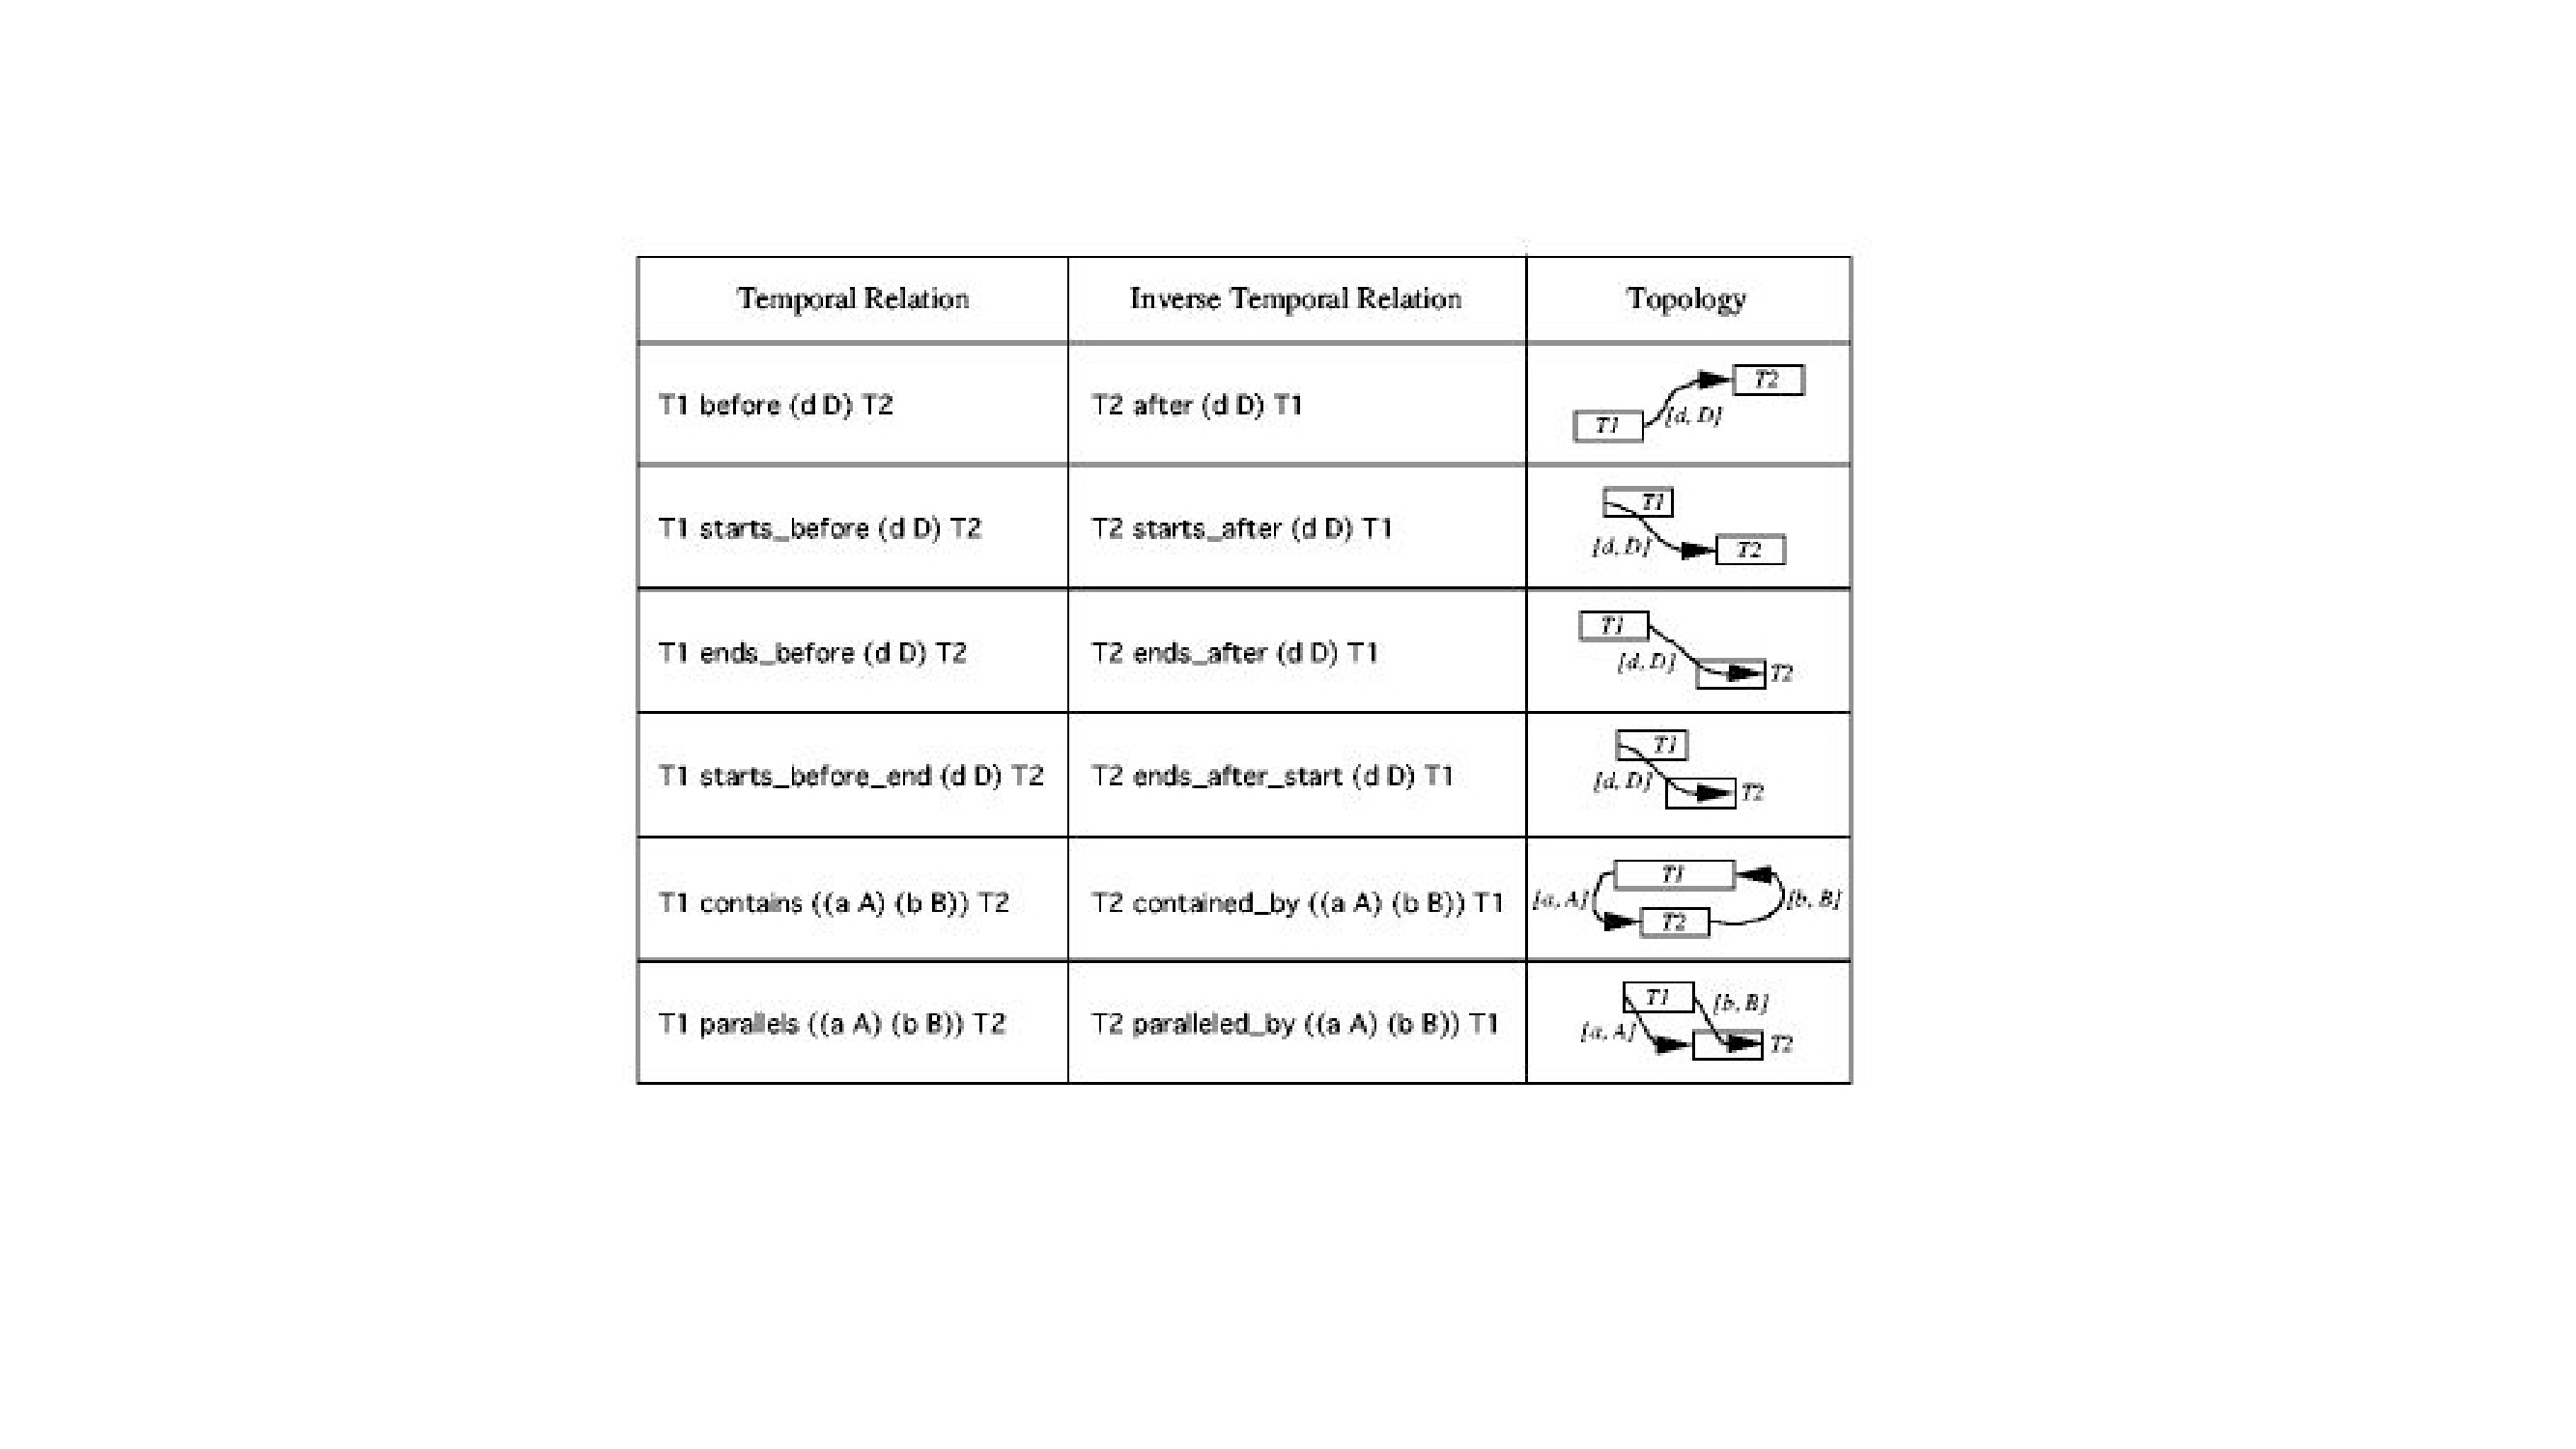
\includegraphics[scale=0.3]{figs/Allen-algebra.pdf}
\caption{\small Temporal relations defined within the planner are
  based on \texttt{Allen Algebra} relations shown above.}
\label{fig:allen-algebra}
\vskip-0.3cm
\end{figure}
 
Each of the token variables, including the parameter variables, has a
domain of values assigned to it.  The variables may also participate
in constraints that specify which value combinations are valid.  To
allow the specification of multiple values, e.g, to express a range of
possible start times, variables are used to specify parameter, start
and end time values for a token.  As a result, a token $T$ is a tuple
$\langle v, P, s, e \rangle$, where $v$ is a variable denoting a state
variable, $P$ is the name of a procedure and $s$ and $e$ (satisfying
$s\leq e$) are variables encoded as flexible token start and end time
points. Consequently, partial plans represent a \textit{range of
  possible solutions} rather than an explicit definition of a single
trajectory of state.  Fig. \ref{fig:flex-timelines} shows an example
of a part of such plans with tokens representing constraints on
flexible temporal intervals. Systematic computation is reflected by
the use of the \texttt{Allen Algebra} \cite{allen84} temporal
relations shown in Fig. \ref{fig:allen-algebra}. It is the use of such
interval arithmetic in the \eu domain model that allows
encoding of temporal constraint relationships between tokens on the
same or other concurrent timelines. Details of propagation algorithms
or of interval logic are beyond the scope of this paper.

\begin{figure}
\centering
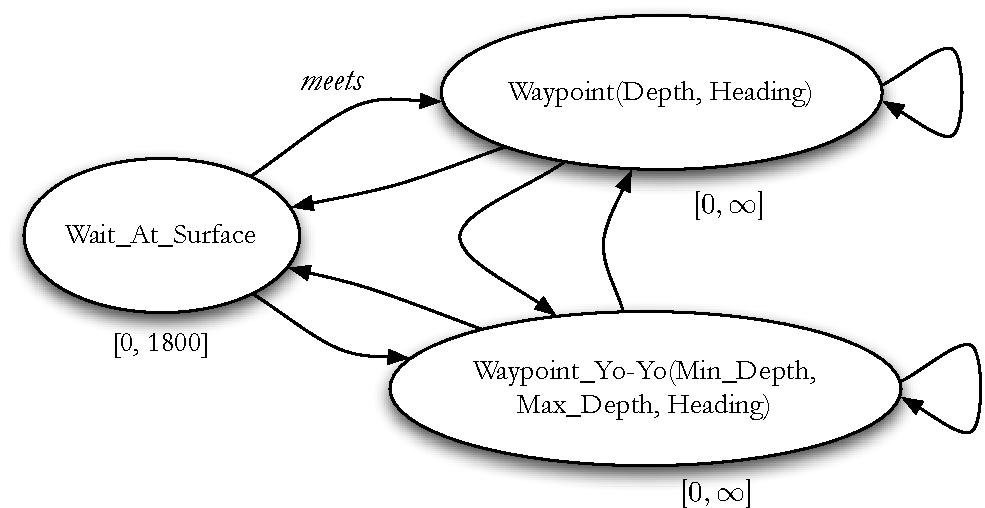
\includegraphics[scale=0.3]{figs/FSM-transition.pdf}
\caption{\small Timeline evolution can be described by simple finite
  state transitions where temporal relationships describe the arc
  transition and temporal extant of state are token
  durations. Constraints here are for \emph{meets} or its equivalent
  inverse \emph{met\_by}.}
\label{fig:FSM}
\vskip-0.3cm
\end{figure}

In describing the evolution of state via timelines, transitions within
a timeline can be described by simple finite state
machines. Fig. \ref{fig:FSM} for example describes a timeline
evolution for an abstract timeline entity describing navigation. Arc
transitions represent temporal constraints and token duration are
represented by temporal extant of state. The entire vehicle can then
be modeled as a number of state transitions with concurrency for each
of the modeled state variables defined a priori. However this simple
view is often complicated when temporal constraints between state
variables are articulated in our domain models. If there is a
criticism of this approach, modeling then, requires a proper balance
between abstraction, state variable description and concurrency
described by the inter-connectedness between such finite state
machines. 


\begin{figure*}
\centering 
\subfloat[]{\label{fig:plan-evolve1}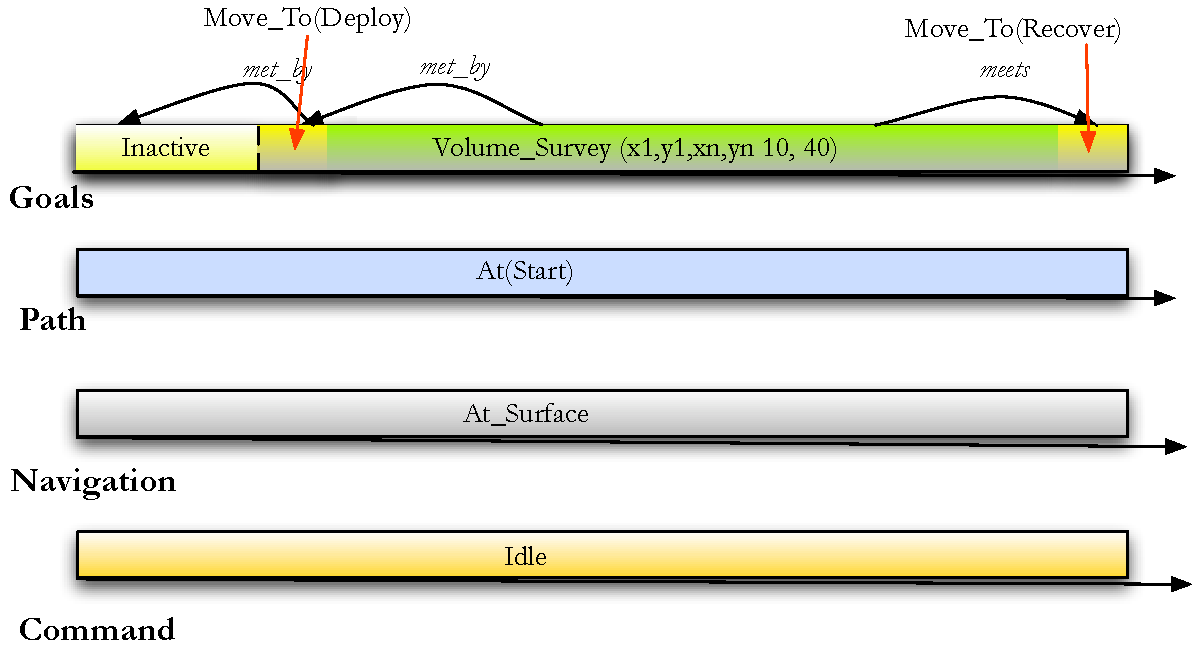
\includegraphics[width=0.3\textwidth]{figs/Plan-evolve-1.pdf}} 
\subfloat[]{\label{fig:plan-evolve2}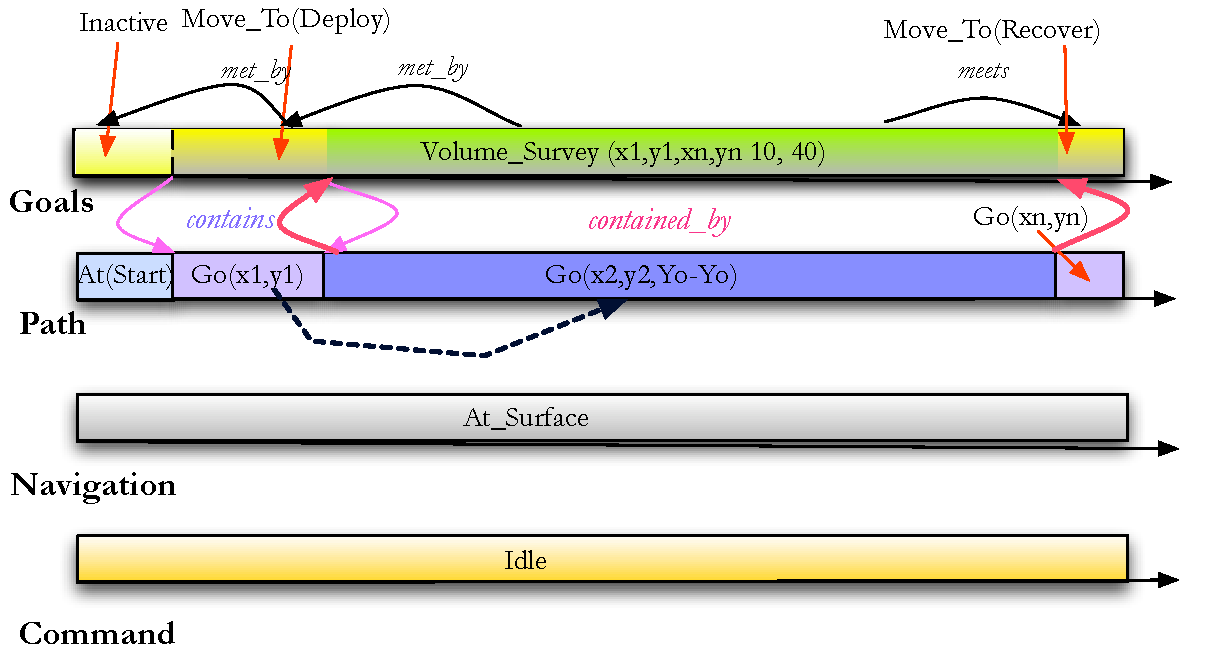
\includegraphics[width=0.3\textwidth]{figs/Plan-evolve-2.pdf}} 
\subfloat[]{\label{fig:plan-evolve3}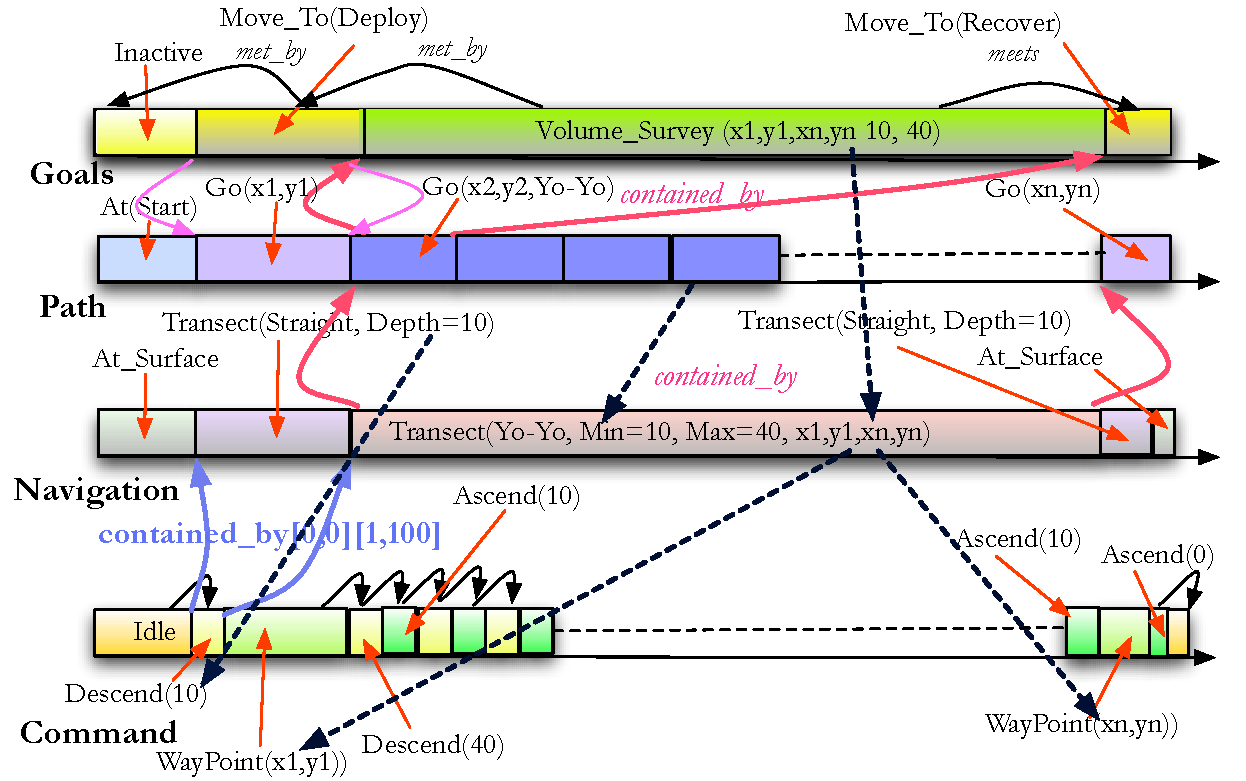
\includegraphics[width=0.3\textwidth]{figs/Plan-evolve-3.pdf}} 
\caption{\small An illustrative plan synthesis example with concurrent
  timelines. Each timeline is an instantiation of a subsystem tracked
  by the planner. Tokens describe the instantiated state of subsystem
  at a particular time instance and enforce temporal and parametric
  constraints. Abstract goals are decomoposed into successively less
  abstract tokens and instantiated in co-temporal timelines using
  \texttt{Allen Algebra} relations. All tokens represent flexible
  start/end times. \ref{fig:plan-evolve1} shows an initial state
  evolving into \ref{fig:plan-evolve2} and \ref{fig:plan-evolve3}.}
  \label{fig:Plan-evolve}
  \vskip-5pt
\end{figure*}

Fig. \ref{fig:Plan-evolve} shows an illustrative example. We show four
timelines which track \texttt{Goal, Path, Navigation} and
\texttt{Command} state over time. Tokens on the goal timeline indicate
a survey within a bounded volume and a min/max depth envelope. As the
Volume Survey sub-goals on the \texttt{Path} timeline, the initial
token on that timeline gets \emph{squeezed} to have dependencies of
the goal token instantiated. Initially this dependency are the tokens
\texttt{Go(x1,y1)} and \texttt{Go(xn,yn)} indicative of the area of
coverage. The first of these in turn generates a sub-goal on the same
timeline to go to the next intermediate waypoint, which is illustrated
in Fig. \ref{fig:plan-evolve2}. Subsequent sub-goals (not shown in the
figure) ultimately generate all the tokens to completion for this
timeline. Fig. \ref {fig:plan-evolve3} shows a snapshot further along
in plan generation and shows additional subgoals on the \texttt{Path,
  Navigation} and \texttt{Command} timelines. Each token can thus
trace its causality when instantiated in the plan. The domain model
provides source of these temporal and parametric dependencies in the
form of rules. 

\begin{minipage}[c]{\textwidth}
\vspace{+0.5cm}
% \framebox[\textwidth][t]{
Volume\_Survey(x$_1$,y$_1$,x$_n$,y$_n$,Min\_Depth, Max\_Depth)\\
$\Rightarrow$ \\
met\_by Go(x$_1$,y$_1$,Min\_Depth); \\
starts [50,0] Go(x$_2$,y$_2$,Min\_Depth,Max\_Depth); \\
\ldots{} \\
ends [50,0] Go(x$_{n-1}$,y$_{n-1}$, Min\_Depth,Max\_Depth); \\
meets Go(x$_n$,y$_n$,Min\_Depth, Max\_Depth); 
\end{minipage}


% \subsubsection{Partitioned Control}


% \subsubsection{State Estimation}

% Even as automated reasoning approaches have the ability to dynamically
% retarget the vehicle, estimating environmental signals of interest (or
% their proxies) is important to be able to enable opportunistic science
% in the water-column. In \texttt{T-REX} feature recognition revolves
% around a Hidden Markov Model (HMM) \cite{rabiner86} which is encoded
% directly within the unified representational and computational
% framework of a reactor. HMMs are useful since the stochastic nature of
% these models can correlate the type of features we want to detect with
% the sensor observations. Online targeted sensor data is classified by
% apriori generated cluster data which in turn determines the
% probability of having seen the feature of interest. Together with
% posterior probability, the HMM generates a probability of being within
% the target feature if it dominates the distribution. If other sampling
% conditions are satisfied (for instance sampling proximity), a
% constraint is activited in the model which can trigger a water sampler
% and also preserve the memory of sampling to alter a future transect
% resolution.


% The HMM is customized for the feature of interest and is built offline
% using clustering techniques from large data sets; we use Kohonen's
% Self Organizing Maps \cite{kohonen}. We use a semi-supervised learning
% method \cite{zhu05} to extract an environmental model that make uses
% of both labeled and unlabeled data for training. Online,

% The sensor data for classification depends on the
% feature of interest; for detecting INLs we use backscattering data
% from a HydroScat and for tracking riverine plumes to track fertilizer
% runoff, we use an ISUS Nitrate sensor.

%%% Local Variables: 
%%% mode: latex
%%% TeX-master: "ieee-ram09"
%%% End: 
